\documentclass[notheorems]{beamer}
\usetheme{Lab2C}
\usepackage{graphicx}
\usepackage{subcaption}
\newif\ifbeamer
\beamertrue

\title{Reproducing Scientific Experiment with Cloud DevOps}
\author{Feng Zhao}
%\institute{\inst{1}Dept. of Electronic Engineering, Tsinghua University
%\and \inst{2}Tsinghua-Berkeley Shenzhen Institute, Tsinghua University}
\date{\today}
\begin{document}
\begin{frame}
	\titlepage
\end{frame}
\section*{Outline}
\begin{frame}
	\tableofcontents
\end{frame}

\section{Introduction}
\begin{frame}
\frametitle{Background}
	\begin{columns}
		\column{5cm}
		\begin{figure}
			
\includegraphics[width=4cm]{pic/cloud_computing.png}
		\end{figure}
		\column{5cm}
	Cloud Computing is 	a promise field of future computing platform.
		\end{columns}
\begin{figure}
	\centering
	\begin{subfigure}{0.33\textwidth}
		
\includegraphics[width=\textwidth]{pic/github_actions.png}
		\caption{DevOps workflow}
	\end{subfigure}~~~~~
	\begin{subfigure}{0.33\textwidth}
		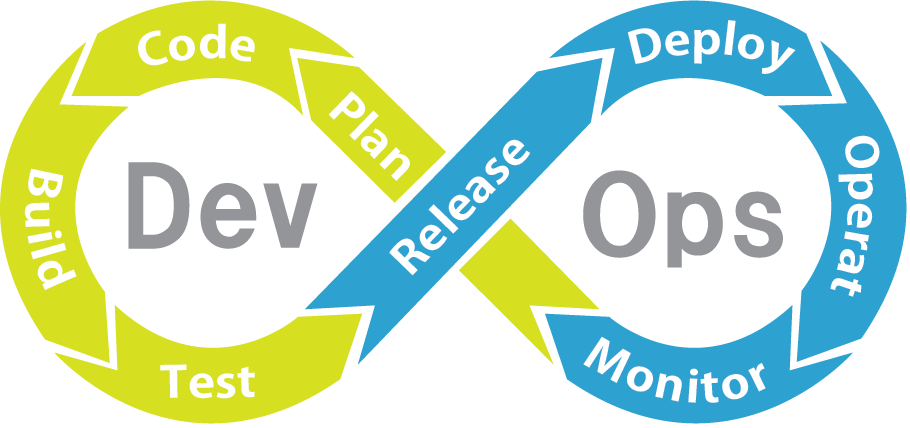
\includegraphics[width=\textwidth]{pic/general_workflow.png}
		\caption{Cloud DevOps provider}
	\end{subfigure}
\end{figure}  
DevOps is a kind of workflow management methodology in software engineering field.
\end{frame}

\begin{frame}
\frametitle{Challenges in Reproducibility}
\begin{itemize}
\item No source code
\item specific hardware requirement
\item specific software requirement
\item complex workflow not clear to others
\end{itemize}
source code of one Nature article gave different results on different Operating Systems.

{\tiny J.~Bhandari~Neupane, R.~P. Neupane, Y.~Luo, W.~Y. Yoshida, R.~Sun, and P.~G.
  Williams, ``Characterization of leptazolines a--d, polar oxazolines from the
  cyanobacterium leptolyngbya sp., reveals a glitch with the
  “willoughby--hoye” scripts for calculating nmr chemical shifts,''
  \emph{Organic Letters}, 2019.
 } 
 
\end{frame}

\begin{frame}
\frametitle{Existing Method}
specific software tools
\begin{figure}
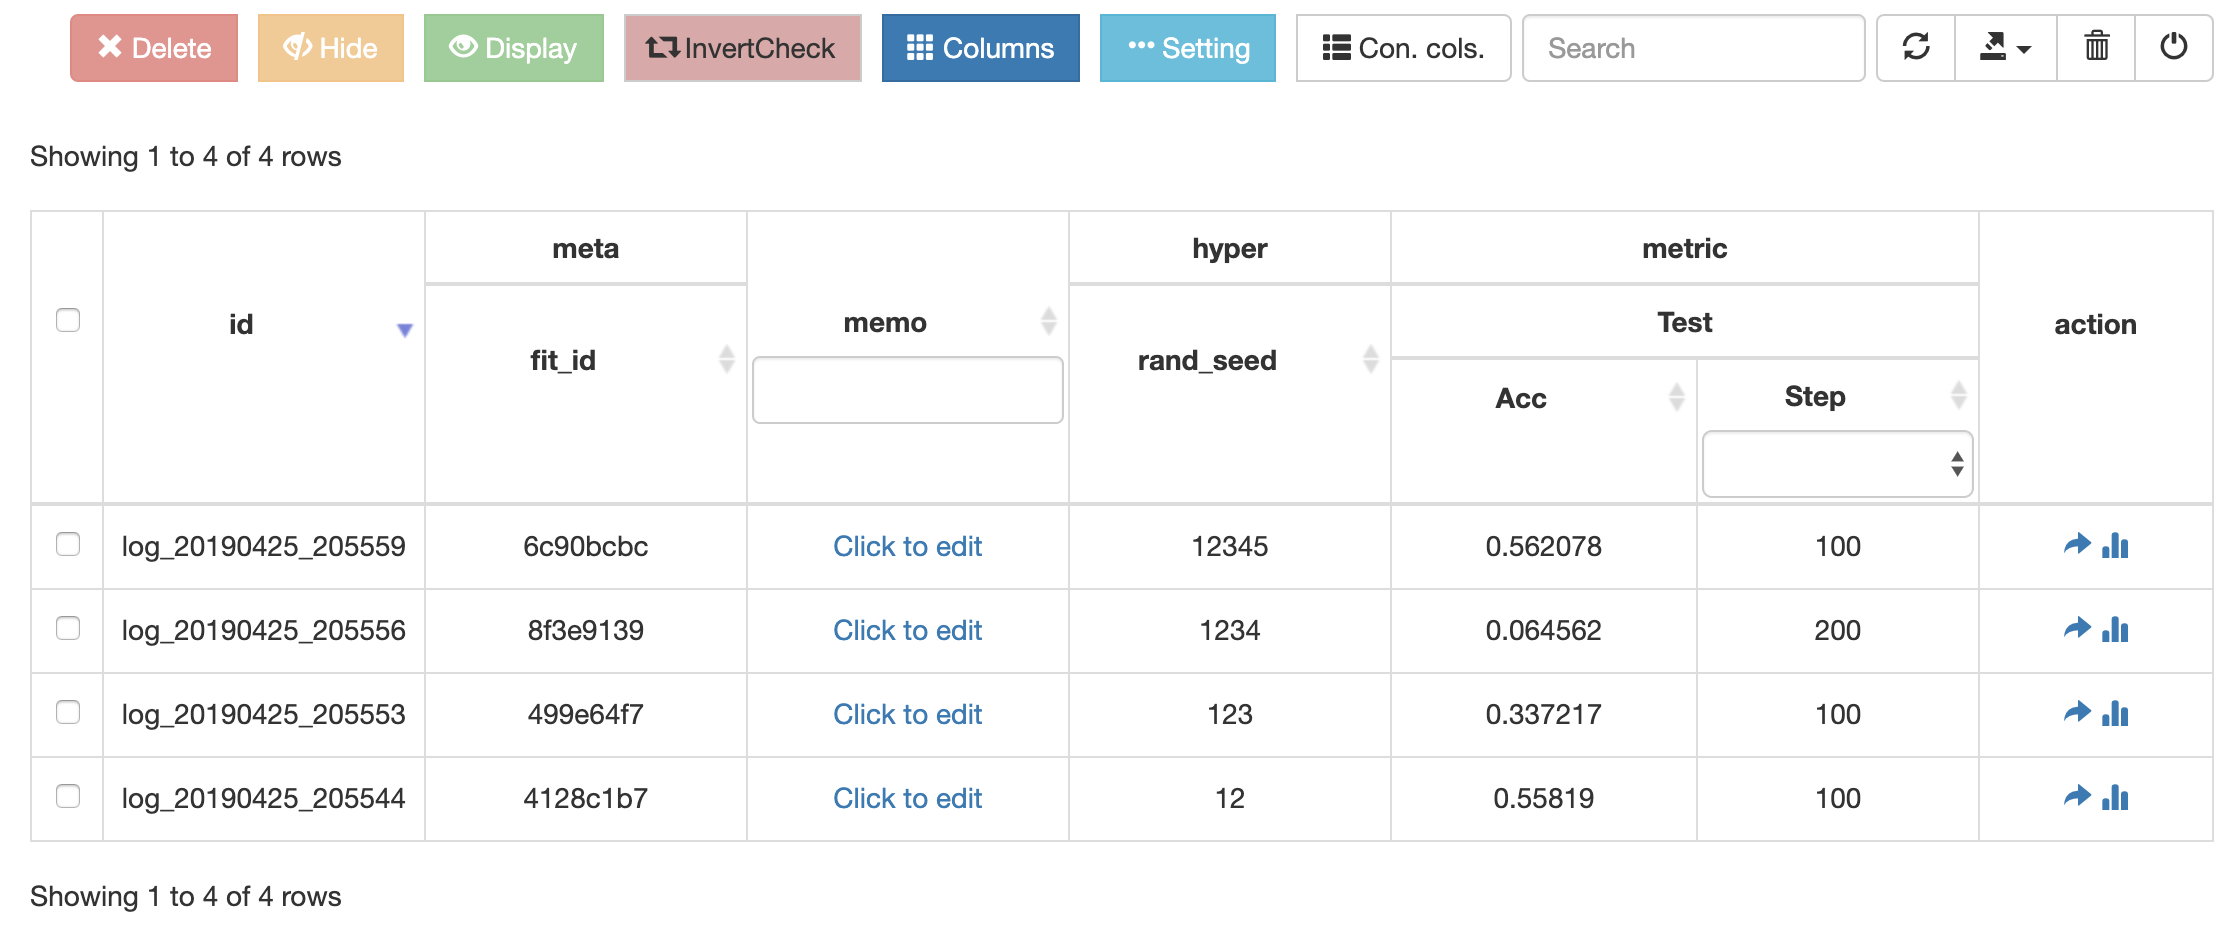
\includegraphics[width=5cm]{pic/fitlog_table.png}
\end{figure}
Pros: running environment information capture and experiment results storage

Cons: bad maintainability and difficult configuration
\end{frame}

\begin{frame}
	\frametitle{Existing Method}
Out-of-box Platforms
\begin{figure}
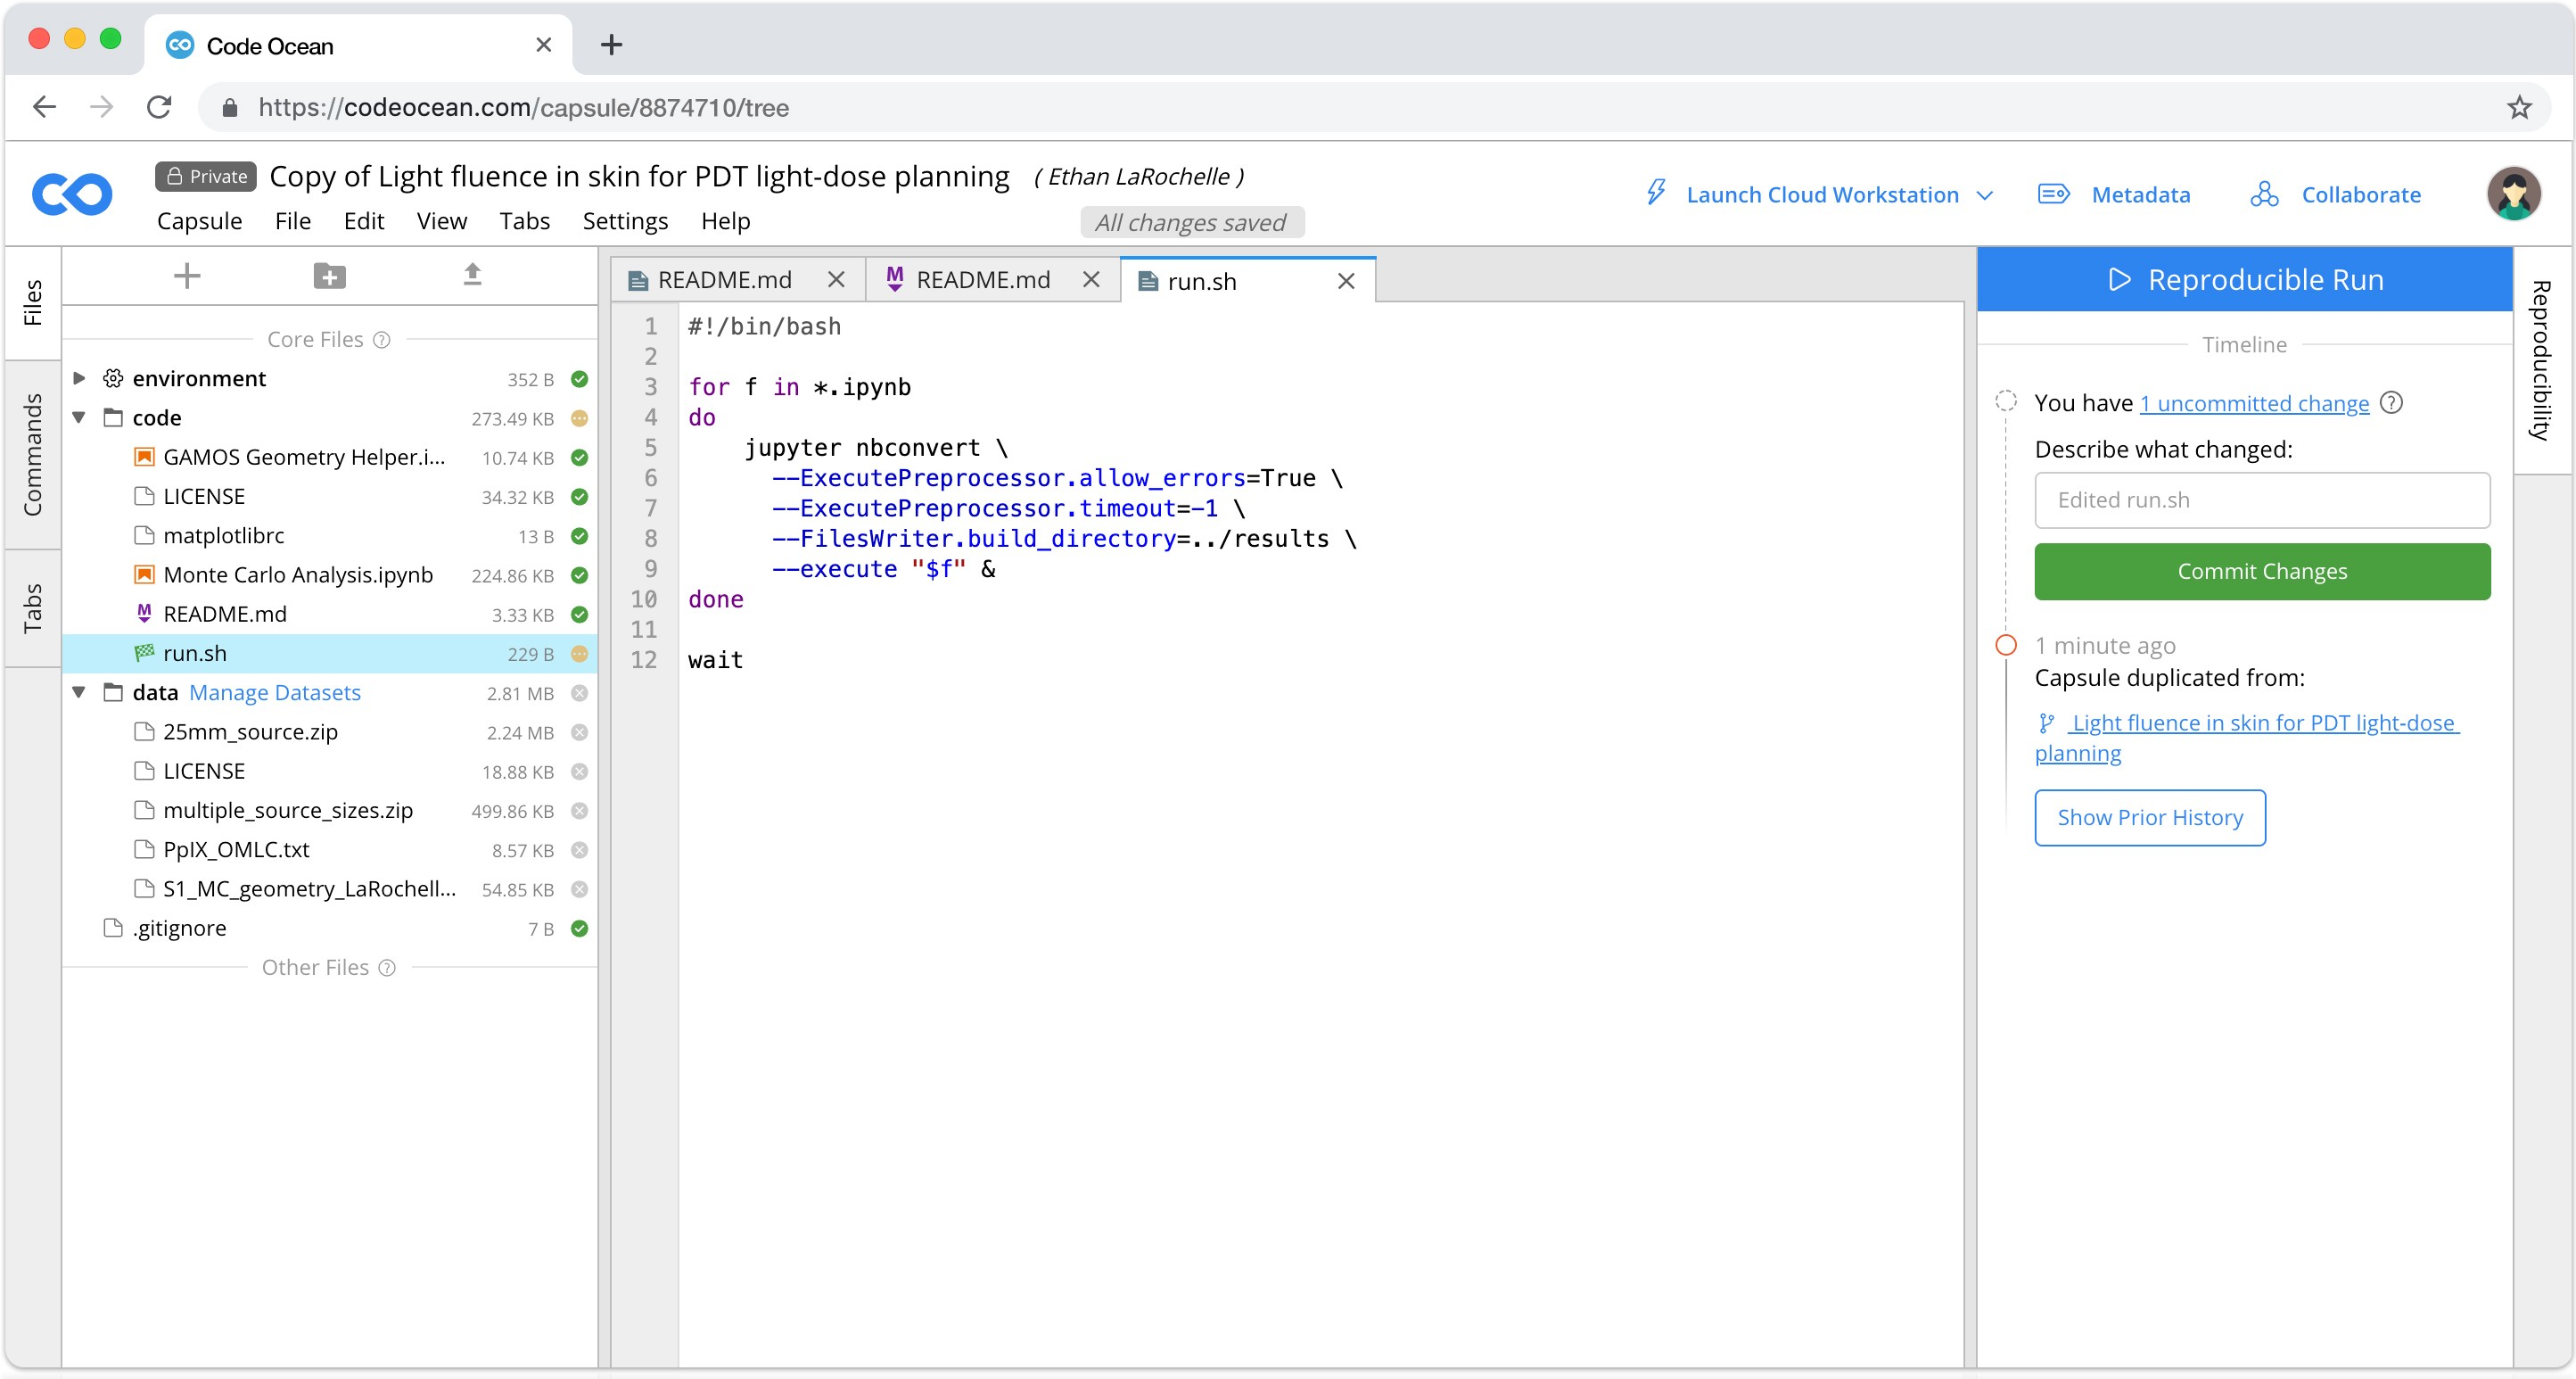
\includegraphics[width=5cm]{pic/code_ocean.jpeg}
\end{figure}
Pros: Uniform platform and easy to use

Cons: pay for your usage
\end{frame}

\begin{frame}
\frametitle{Existing Method}
Best practice

Make documentation of experiment procedures, etc.

Pros: no external barrier

Cons: varies between researchers
\end{frame}
\section{Infrastructure}
\section{Experiments}
\section{Conclusion}
\begin{frame}
\frametitle{Conclusion}
\begin{itemize}
\item Formulate Info-Detection method
\item Propose improved principal sequence of partition algorithm 
\item Demonstrate Info-Detection performs well on some datasets
\end{itemize}
\end{frame}
\begin{frame}
\frametitle{}
\begin{block}{}
\centering
Thank you!
\end{block}
\end{frame}
\end{document}
